\chapter{Conclusioni}
Dai risultati raccolti e presentati nel precedente capitolo è evidente la differenza di accuratezza raggiunta sui due dataset. In particolare, nonostante si riesca facilmente ad ottenere un modello con risultati buoni o ottimi sul dataset WESAD, ciò non è stato ottenuto sul dataset ASCERTAIN originale mentre si hanno risultati sensibilmente migliori sullo stesso dataset ASCERTAIN modificato rendendo ogni soggetto più bilanciato riguardo le classi contenute.

% traccia possibile \/
% differenza wesad -- ascertain -> cosa rende risultati su wesad così migliori?
% importanza del bilanciamento dei dati
% approcci continui ottimi a seconda dei dati
% approcci che allo stato attuale sembrano funzionare meglio rispetto alla tipologia di dati
% applicabilità future a seconda dei dati disponibili

\section{Differenze fra i due dataset}
Uno degli elementi da considerare quando si addestra una rete neurale è il bilanciamento dei dati presi in considerazione per l'addestramento.
Andando ad analizzare nel dettaglio la struttura dei due dataset considerati, diventa evidente la decisa sovrarappresentanza della classe 0 nel dataset ASCERTAIN, mentre le classi nel dataset WESAD risultano molto più bilanciate. Questo è anche dovuto all'aver scelto delle classi fittizie, per quanto riguarda ASCERTAIN, che ha evidenziato come non tutti i soggetti abbiano prodotto dati bilanciati rispetto alle nuove classi selezionate.\\\\
Bilanciando il dataset ASCERTAIN attraverso la produzione di soggetti fittizi, ognuno contenente dati presi da tutti i soggetti in maniera bilanciata rispetto alle nuove classi, otteniamo immediatamente risultati sensibilmente migliori, con accuratezze a volte anche doppie rispetto allo stesso approccio sul dataset ASCERTAIN originale. Questo rende evidente l'importanza dell'avere dati di addestramento bilanciati, quindi esempi in quantità simile per ogni etichetta possibile.
\begin{figure}[h]
    \begin{minipage}[b]{0.5\textwidth}
		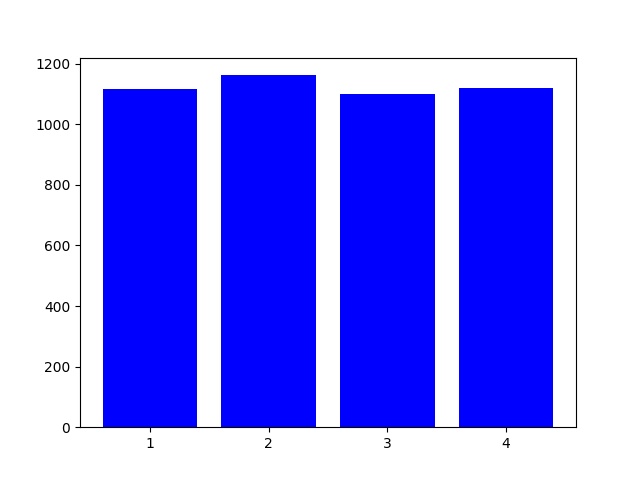
\includegraphics[width=\textwidth]{img/graphs/wesad_dataset.png}
		\caption{Presenza delle classi su dataset WESAD}
		\label{fig:wesadclasses}
	\end{minipage}
    \hfill
    \begin{minipage}[b]{0.5\textwidth}
		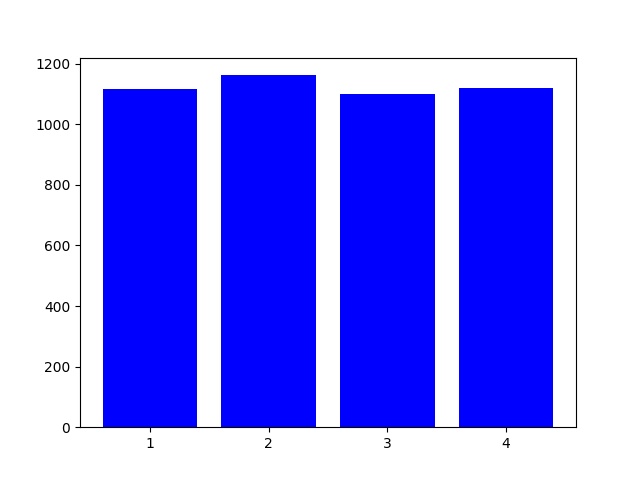
\includegraphics[width=\textwidth]{img/graphs/wesad_dataset.png}  % TODO
		\caption{Presenza delle classi su dataset ASCERTAIN}
		\label{fig:ascertainclasses}
	\end{minipage}
\end{figure}

\section{Approcci continui a confronto}
Dai risultati ottenuti e elencati nelle tabelle \ref{tab:reswesad}, \ref{tab:resascertain} e \ref{tab:rescustomascertain} possiamo mettere a confronto fra loro i diversi approcci di continual learning presi in considerazione.